\subsection{Participate}
Im Bezug auf Verwendbarkeit wie in Kap. \myRefGeneral{sec:UserJourney} beschrieben ist, soll die Startseite die \emph{Participate}-Seite sein. 
In dieser soll der Benutzer bzw. Student der an einer Umfrage teilnimmt, einen \emph{Surveycode} wie z.B. \emph{\texttt{OYZQGGXOF9}} eingeben, um an der Umfrage zu partizipieren. 

Anschließend wird der Benutzer auf die Umfrageseite weitergeleitet, auf der er die benötigten Felder ausfüllt (siehe Kap. \vref{ssec:UmfrageImplement}).

\begin{figure}[hp]
	\centering
	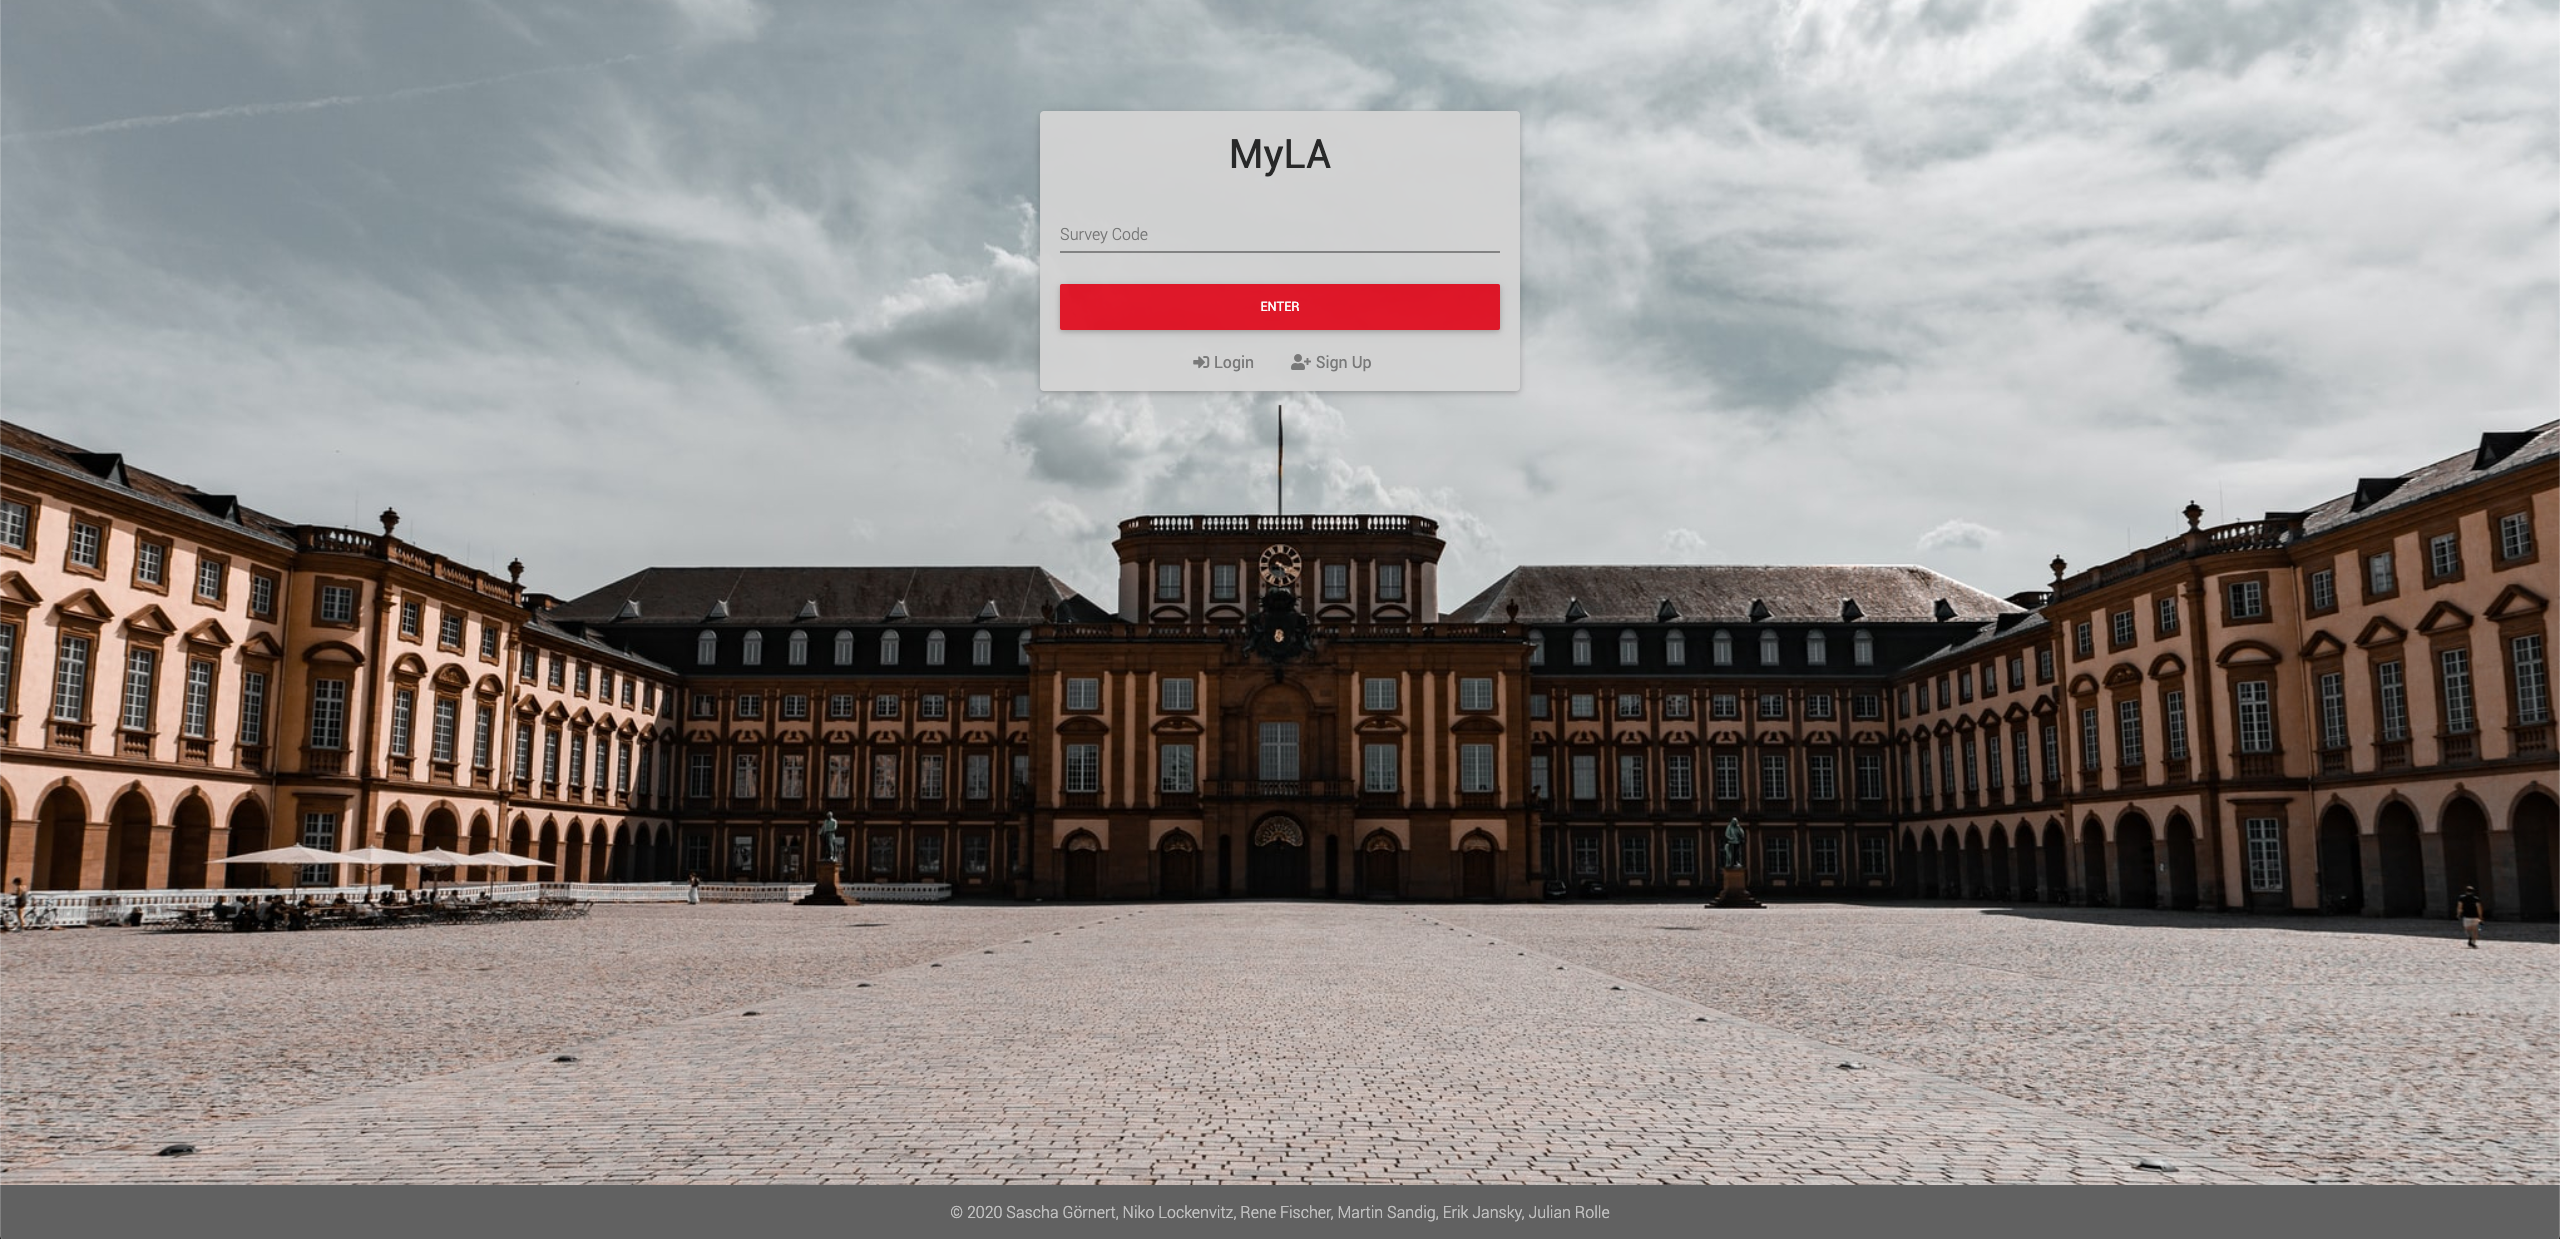
\includegraphics[width=0.95\textwidth, keepaspectratio]{img/client/Participate.png}
	\captionsetup{justification=centering, format=plain}
	\caption[\acf{UI}: Teilnahme Umfrage]{\acf{UI}: Teilnahme Umfrage \\ \quelleScreenshot}
	\label{fig:ParticipateImplement}
\end{figure}